% !TeX root = ./main.tex
We now experimentally validate the the performance of the different version of our algorithms for explaining satisfiable constraint satisfaction problems.

We consider the following benchmarks: CNF instances from the SATLIB problems Benchmark \cite{hoos2000satlib} and a CNF encoding of the logic grid puzzle ``Origin'' of \citet{ecai/BogaertsGCG20}. All code was implemented in Python on top of %CPpy~\footnote{} and
PySAT~\footnote{\url{https://pysathq.github.io}}. The MIP solver used is Gurobi 9.0 and when a MaxSAT solver is used it is RC2 as bundled with PySAT. Experiments were run on a Intel(R) Xeon(R) CPU E3-1225 with 4 cores and 32 Gb memory, running linux 4.15.0.

Based on the theoretical findings of the previous sections, we aim to answer the following questions:
\begin{compactitem}
\item RQ1: what is the effect of postponing optimal hitting set computation, of incremental OUS solving and of pre-seeding the MCSs when solving multiple variants of the same problem?
\item RQ2: how do the different variants of \omus perform when explaining an elaborate constraint satisfaction problem?
\item RQ3: how do the sequences found when using (constrained) \omus search compare to those found using a heurisic MUS approach?
\end{compactitem}

\ignore{\color{red}Terminology: 
\begin{itemize}
  \item Postponing optimization = davies
  \item Incremental = Section 6
  \item Constrained = Section 7
  \item Pre-Seeding 
\end{itemize}
No ``delaying propagation''!}

\paragraph{RQ1}
To answer the first research question, we use 10 CNF instances from the SATLIB Benchmark and randomly choose a subset of 10 decision variables. For each variant of the algorithm, we compute the OUS of the same 10 decision variables in the same order within a time limit of 10 minutes. We compare the following enhancements options to the basic \omus algorithm: postponing optimization (+P), incrementality by reusing satisfiable subsets between \omus calls (+I), and pre-seeding $\m{SS}$s from every negated decision variable of the instance (+W). Options can be combined, for example \omus+IPW characterises running the \omus algorithm postponing the optimization phase, with incrementality between the succesive calls, and warm starting with satisfiable subsets of the original CNF formula.
%The executions are set to timeout after 10 minutes, a limit fixed based on the results of experiment 2.

% \rule{\textwidth}{10pt}

\begin{table*}[t!]
    \centering
    \begin{tabular}{|c|c|c|c|c|c|c|c|c|}
        \hline
        % p    & nv& nc&           \omus &      \omus+Incr &      \omus+Post &  \omus+Incr+Warm &   \omus+Incr+Post & \omus+Incr+Post+Warm \\
        p    & nv& nc&           \omus &      \omus+I &      \omus+P &  \omus+IW &   \omus+IP & \omus+IPW \\
        \hline
        1 & 50& 80&   0.88 s  &   0.38 s  &   0.37 s  &   0.81 s  &    0.65 s  &      \textbf{0.33} s  \\
        2 & 350 & 1157 &   122.42 s  &  94.07 s  &  96.84 s  &  120.55 s  &  126.15 s  &     \textbf{87.31} s  \\
        3 & 155& 1135&   130.38 s  &  87.97 s  &  84.75 s  &  104.7 s  &  124.48 s  &     \textbf{80.92 s}  \\
        4  & 1015 & 3324&      --- &     --- &     --- &     --- &      --- &        --- \\
        % 5 & 317 & 1264           &      --- &  --- &  --- &     --- &      --- &     --- \\
        % 6 & 324 & 1292        &      --- &     --- &     --- &     --- &      --- &        --- \\
        % 7 & 334 & 1332        &      --- &     --- &     --- &     --- &      --- &        --- \\
        % 8& 349 & 1392         &      --- &     --- &     --- &     --- &      --- &        --- \\
        % 9  & 1015 & 3324        &      --- &     --- &     --- &     --- &      --- &        --- \\
        % 10  & 718 & 4934       &      --- &     --- &     --- &     --- &      --- &        --- \\
        \hline
        \end{tabular}
        \caption{Comparison of \omus variants evaluated on CNF instances.}
        \label{table:experiment1}
\end{table*}

% \begin{table*}[t!]
%     \centering
%     \begin{tabular}{c|cccc|cccccc}
%         % \hline
%         p &  time [s] &  \#steps &   $\overline{cost}$ & max(cost) &    1 bij &  1trans &  1 clue & 1 clue+i & 1 mult-i & mult-c. \\
%         \hline
%         1 &  1287.27 &     115 &     25.87  &    25.87  &  31.83\% &  50.57\% &  1.09\% &    16.52 \% &     0\% &    0.0\% \\
%         % \hline
%         \end{tabular}
%         \caption{Puzzle Properties, execution statistics and explanation sequence composition for the origin puzzle.}
%         \label{table:experiment3}
% \end{table*}

% ------------------------------- EMILIO LOCK -----------------------------------------
The results can be seen in Table \ref{table:experiment1} and can be summarized as follows: p, nv and nc represent the instance name, the number of variables and the number of clauses respectively. 
Only for instances 1 (aim-50-1\_6-yes1-4.cnf), 2 (par8-2.cnf) and 3 (zebra\_v155\_c1135.cnf), is the algorithm able to complete the search for \texttt{OUS}s on the 10 decision variables within the required time constraint of 10 minutes.
All variants time out on the larger instances finding the \texttt{OUS}s up to 6 out of the 10 decision variables.
%\tias{remove other ones, say that larger instances timed out in the text}
A further analysis of the overall execution times highlights that the main bottleneck of the algorithm is the time spent \todo{emilio} $\m{SS}$s
\tias{in general or for warmstarting? This means that my 'implementation consideration' of using a MaxSat solver is cheap is not true...}. For instances 1-3 executed without postponing optimization, \todo{ emilio}\% of the time is spent growing, and for the remaining instances close to \todo{ emilio} \% of the time is spent \todo{ emilio} .
In particular, for executions involving postponing the calls (+P/+IP/+IPW) to the MIP solver, \todo{ emilio}\% of the time is spent growing, while the remainder of the time is distributed between incremental and greedy computation of hitting sets.
Finally, we conclude that within the short time limit provided, the best configuration for computing multiple related OUS's is \omus+IPW, taking advantage of the repeated calls to the OUS algorithm, thus reusing the computed $\m{SS}$s.
% ------------------------------- EMILIO LOCK -----------------------------------------

% \begin{table*}[h!]
%     \begin{tabular}{|c|c|c|c|c|c|c|c|c|}
%         \hline
%         % p    & nv& nc&           \omus &      \omus+Incr &      \omus+Post &  \omus+Incr+Warm &   \omus+Incr+Post & \omus+Incr+Post+Warm \\
%         p    & nv& nc&           \omus &      \omus+I &      \omus+P &  \omus+IW &   \omus+IP & \omus+IPW \\
%         \hline
%         1 & 50& 80&   0.88 s  &   0.38 s  &   0.27 s  &   0.81 s  &    0.65 s  &      0.33 s  \\
%         2 & 350 & 1157 &   22.42 s  &  14.07 s  &  76.84 s  &  20.55 s  &  126.15 s  &     87.31 s  \\
%         3 & 155& 1135&   130.38 s  &  87.97 s  &  64.75 s  &  104.7 s  &  124.48 s  &     80.92 s  \\
%         4..10 & x $\cdot$ $10^2$ & x $\cdot$ $10^3$           &      --- &     --- &   --- &  --- &   --- &     --- \\
%         % 5 & 317 & 1264           &      --- &  --- &  --- &     --- &      --- &     --- \\
%         % 6 & 324 & 1292        &      --- &     --- &     --- &     --- &      --- &        --- \\
%         % 7 & 334 & 1332        &      --- &     --- &     --- &     --- &      --- &        --- \\
%         % 8& 349 & 1392         &      --- &     --- &     --- &     --- &      --- &        --- \\
%         % 9  & 1015 & 3324        &      --- &     --- &     --- &     --- &      --- &        --- \\
%         % 10  & 718 & 4934       &      --- &     --- &     --- &     --- &      --- &        --- \\
%         \hline
%         \end{tabular}
%         \caption{Comparison of \omus variants evaluated on CNF instances.}
%         \label{table:experiment1}
% \end{table*}

% \begin{table*}
%     \begin{tabular}{|c|c|c|c|c|c|c|}
%         \hline
%         p                  &           \omus &      \omus+Incr &      \omus+Post &  \omus+Incr+Warm &   \omus+Incr+Post & \omus+Incr+Post+Warm \\
%         \hline
%         1 &    0.88 s | 10 &   0.38 s | 10 &   0.27 s | 10 &   0.81 s | 10 &    0.65 s | 10 &      0.33 s | 10 \\
%         2            &   22.42 s | 10 &  14.07 s | 10 &  76.84 s | 10 &  20.55 s | 10 &  126.15 s | 10 &     87.31 s | 10 \\
%         3  &  130.38 s | 10 &  87.97 s | 10 &  64.75 s | 10 &  154.7 s | 10 &  124.48 s | 10 &     80.92 s | 10 \\
%         4            &      600 s | 1 &  600 s | 2 &  600 s | 1 &     600 s | 1 &      600 s | 1 &     600 s | 1 \\
%         5         &      600 s | 1 &     600 s | 1 &     600 s | 1 &     600 s | 1 &      600 s | 1 &        600 s | 1 \\
%         6         &      600 s | 1 &     600 s | 1 &     600 s | 1 &     600 s | 1 &      600 s | 1 &        600 s | 1 \\
%         7         &      600 s | 1 &     600 s | 1 &     600 s | 1 &     600 s | 1 &      600 s | 1 &        600 s | 1 \\
%         8          &      600 s | 6 &     600 s | 6 &     600 s | 2 &     600 s | 6 &      600 s | 2 &        600 s | 2 \\
%         9         &      600 s | 1 &     600 s | 1 &     600 s | 1 &     600 s | 1 &      600 s | 1 &        600 s | 1 \\
%         10            &      600 s | 6 &     600 s | 6 &   600 s | 6 &  600 s | 6 &   600 s | 6 &     600 s | 6 \\
%         \hline
%         \end{tabular}
%         \caption{Comparison of \omus variants evaluated on CNF instances.}
%         \label{table:experiment1}
% \end{table*}


\paragraph{RQ2}
The second research question is: how do the different variants perform when explaining an elaborate constraint satisfaction problem? The results for the logic grid puzzle called 'origin' is shown in Figure~\ref{fig:exp2}.

\begin{figure}[t]
    \centering
    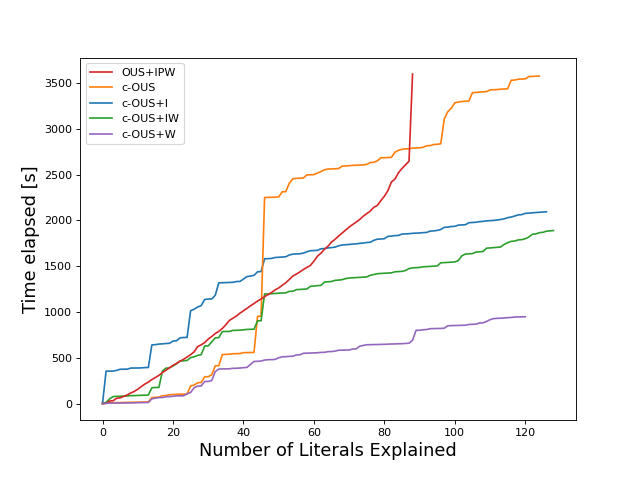
\includegraphics[width=\columnwidth]{figures/omusConstrCumulative.png}
    \caption{Experiment 2}
    \label{fig:exp2}
\end{figure}

The figure shows the number of literals explained on the X-axis, and the cumulative time taken on the Y-axis. 
We can see that OUS-Incremental with pre-seeding and post-poning optimisation is not able to explain all of the literals within the time limit; especially around step 95 there is a big jump in runtime. The vanilla constrained-OUS approach is not able to finish in time either, with big jumps in time on specific (large and costly) explanation steps.

When combining constrained-OUS with either pre-seeding, post-poned optimisation or both, then our approach is able to fully explain the solution. Best results are obtained with constrained-OUS with just pre-seeding at the beginning. The post-poned optimisation in this case may spent a lot of time generating MCSs that are not or little relevant to the constrained OUSs we are seeking.

\paragraph{}
Finally, for \textbf{RQ3} \emilio{Bart: concluding phrases on expl. generation}
%  we compare the sequence found by our proposed method with the sequence reported on in~\cite{ecai/BogaertsGCG20} for the origin puzzle (puzzle 1). 
% The explanation sequence for the puzzle is generated using \omus Constr with pre-seeding and according to the same cost function as Bogaerts et al.~\cite{ecai/BogaertsGCG20}. We report statistics relating to the explanation generation in table~\ref{table:experiment3}.
% Evidently, one of the most important observations is the speed-up provided by \omus Constr. 
% As a matter of fact, the sequence is generated in a bit more than 21 minutes compared to a few (2-3) hours in~\cite{ecai/BogaertsGCG20}, meaning that \omus Constr is 8-10x faster, while also finding the optimal explanations in each step.
% Table \ref{table:experiment3} also reports that the explanation sequence has become easier to understand: the average cost is slightly lower and so is $max(cost)$, the cost of the most difficult explanation in the puzzle. 


% \begin{table*}
%     \begin{tabular}{ccc|ccc|cccccc}
%         % \hline
%         types &  $|dom|$ &  $|grid|$ &  time [s] &  \#steps &    cost &    1 bij &  1trans &  1 clue & 1 clue+i & 1 mult-i & mult-c. \\
%         \hline
%         4 &      5 &     150 &  1287.27 &     115 &        25.87 &  27.83\% &  49.57\% &  6.09\% &    11.3\% &     5.22\% &    0.0\% \\
%         % \hline
%         \end{tabular}
%         \caption{Puzzle Properties, execution statistics and explanation sequence composition for the origin puzzle.}
%         \label{table:experiment3}
% \end{table*}

%
%\begin{figure*}[ht]
%    \centering
%    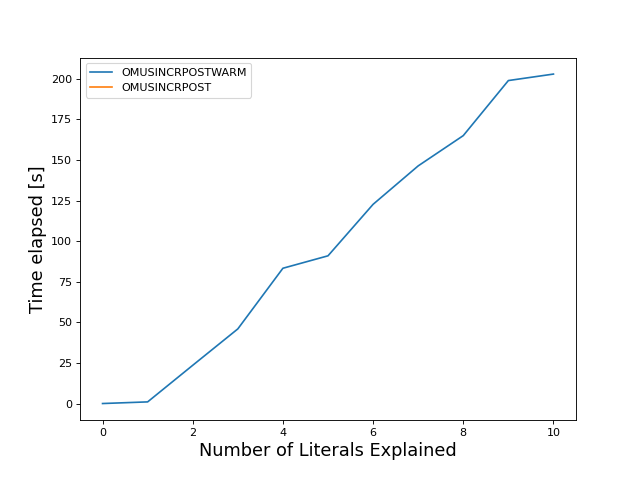
\includegraphics[width=\columnwidth]{figures/omusNonConstrCumulative.png}
%    \caption{}
%    \label{}
%\end{figure*}

% \begin{figure}[ht]
%     \centering
%     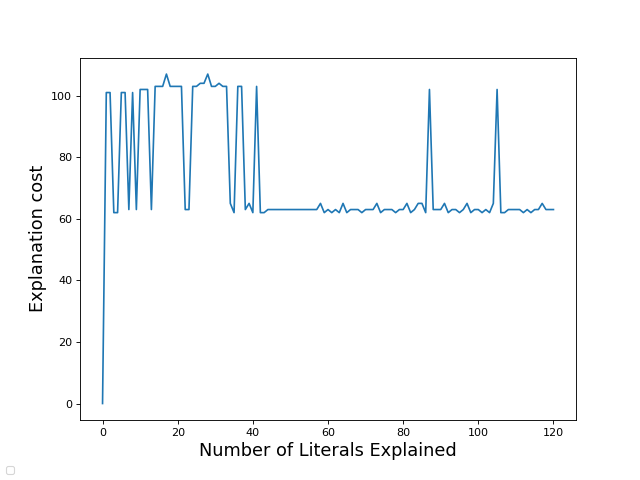
\includegraphics[width=\columnwidth]{figures/explanation_cost.png}
%     \caption{}
%     \label{}
% \end{figure}

